%! TEX program = pdflatex
\documentclass{beamer}

%%% Usepackage
% Basic
\usepackage{amsmath}   % Math input support
\usepackage{amssymb}   % Math input support
\usepackage{booktabs}  % 3 line table show
\usepackage{float}     % Figure and Table env.
\usepackage{makecell}  % Mult. lines in one table cell
\usepackage{bm}

% Color Support
\usepackage{xcolor}
\definecolor{commcolor}{rgb}{0,0.6,0}
\definecolor{rulesepcolor}{rgb}{0.2,0.2,0.2}
\definecolor{stringcolor}{rgb}{0.58,0,0.82}
\definecolor{backcolor}{rgb}{0.93,0.87,0.89}
\definecolor{backcolor2}{rgb}{1,1,0.9}
\definecolor{pergray}{rgb}{0.88,0.88,0.88}

% Coding block
\usepackage{listings}
\lstset{
  language=python,
  basicstyle=\tiny\ttfamily,
  captionpos=b,
  backgroundcolor=\color{backcolor2},
  commentstyle=\color{commcolor},
  escapeinside={\%*}{*)},
  keywordstyle=\color{blue},
  stringstyle=\color{stringcolor}\ttfamily,
  frame=none,
  rulesepcolor=\color{rulesepcolor},
  numbers=left,
  numbersep=4pt,
  numberstyle={\color[RGB]{170,170,170}},
  % xleftmargin=1.5em,
  % xrightmargin=1.5em,
}

% Coding block smooth
\usepackage{tikz}
\usepackage[framemethod=tikz,skipbelow=\topskip,skipabove=\topskip]{mdframed}
\mdfsetup{
  leftmargin=0pt,
  rightmargin=0pt,
  backgroundcolor=backcolor2,
  middlelinecolor=backcolor2,
  roundcorner=5pt,
}
\usepackage{etoolbox}
\BeforeBeginEnvironment{lstlisting}{\begin{mdframed}\vspace{-1em}}
\AfterEndEnvironment{lstlisting}{\vspace{-1em}\end{mdframed}}

% Inline coding
\usepackage{newverbs}
\newverbcommand{\cverb}
  {\setbox\verbbox\hbox\bgroup}
  {\egroup\tcbox{\color{purple}\box\verbbox}}

% Picture shadow box & Inline coding bg
\usepackage[many]{tcolorbox}
\tcbset{
  on line,
  boxsep=0.6pt, 
  left=0pt, right=0pt, top=0pt, bottom=0pt,
  colframe=backcolor, 
  colback=pergray,  
  highlight math style={enhanced}
}


%%% New command
\newcommand{\purple}{\textcolor{purple}}


%%% Page style
\setbeamertemplate{navigation symbols}{}
\usefonttheme{professionalfonts}
\usetheme{Madrid}
\usecolortheme{default}


%%% Pages
%+===================================================================+%
\title[Orbital Magnetization in Solids]{Theory of Orbital Magnetization in Solids}
\subtitle{(Modern Theory of Orbital Magnetization)}

\author[Yang Li]{
  Yang Li\inst{1}}  
\institute[CMT Tsinghua Univ.]{
  \inst{1} Department of Physics\\
           Tsinghua University 
}

\date[Jun. 2021]{Jun. 2021}
%-===================================================================-%

%+===================================================================+%
\AtBeginSection[]
{
  \begin{frame}
    \frametitle{Table of Contents}
    \tableofcontents[currentsection]
  \end{frame} 
}
%-===================================================================-%
 
\begin{document}
  %+===================================================================+%
  \frame{\titlepage}
  %-===================================================================-%

  %+===================================================================+%
  \begin{frame}
    \frametitle{Table of Contents}
    \tableofcontents
  \end{frame}
  %-===================================================================-%

  \section{Brief Review for Magnetization in Solids}
    %+===================================================================+%
    \begin{frame}{Tree of magnetic theory in solids}
      \begin{tcolorbox}[beamer,width=\textwidth,arc=0pt,boxsep=0pt,left=0pt,right=0pt,top=0pt,bottom=0pt]
      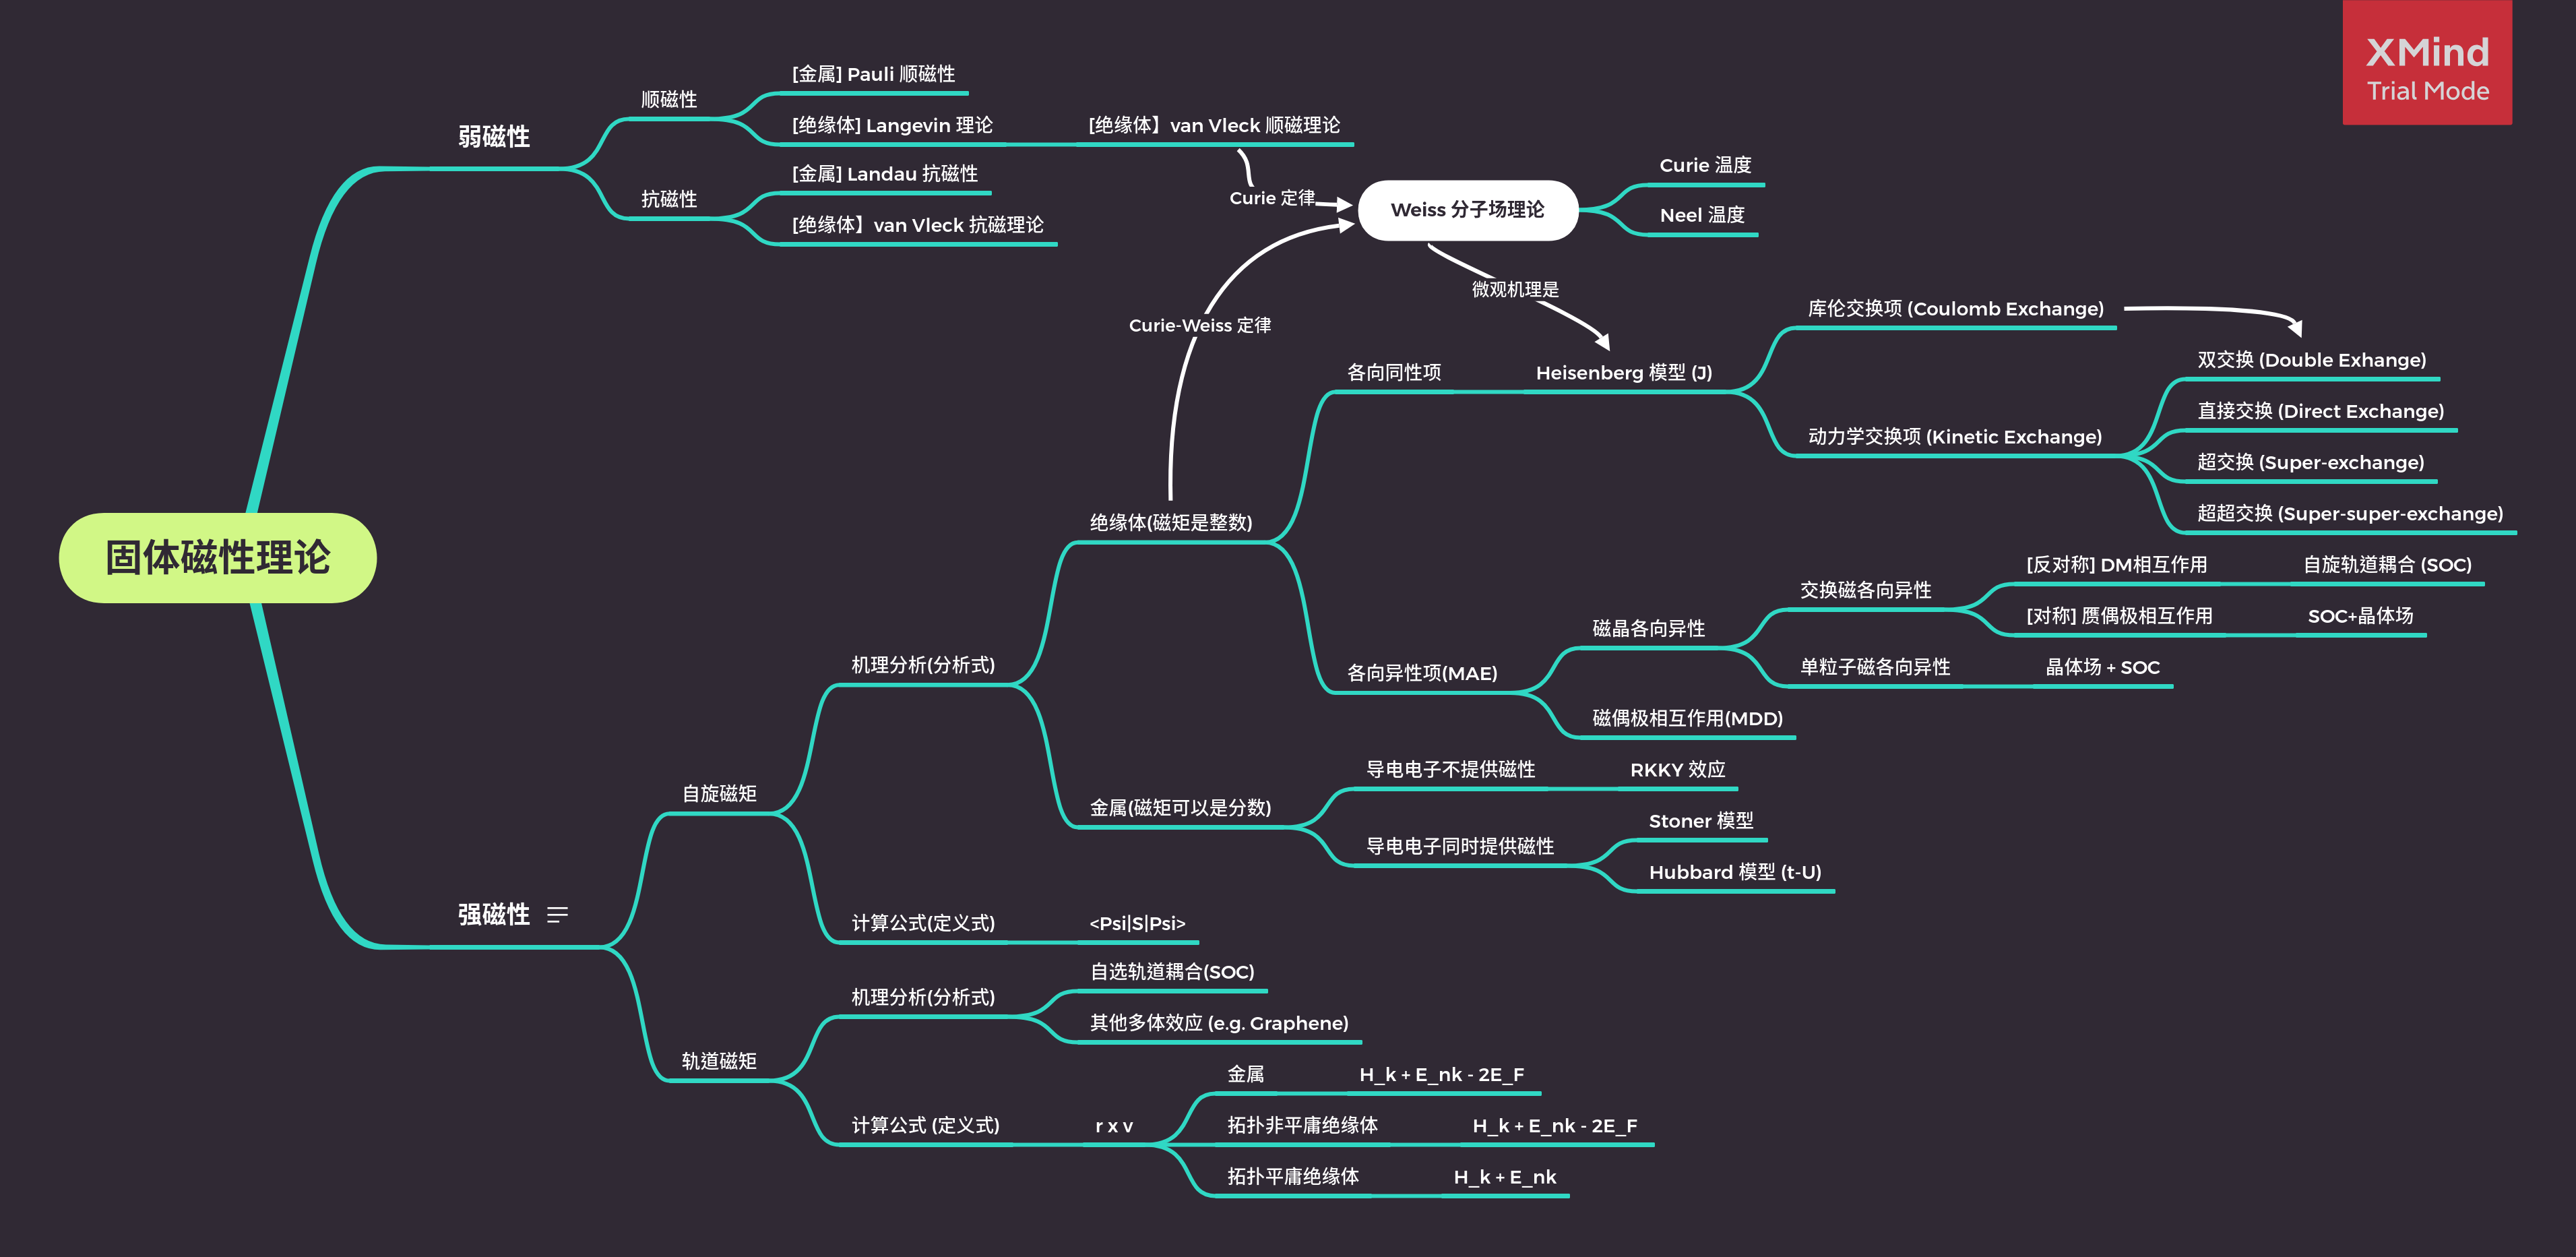
\includegraphics[width=\textwidth]{figure/magnet-tree.png}
      \end{tcolorbox}
      \begin{equation*}
        \bm{M}_{\text{total}} = \bm{M}_{\text{spin}} + \bm{M}_{\text{orb}}
      \end{equation*}
    \end{frame}
    %-===================================================================-% 

    %+===================================================================+%
    \begin{frame}{Why we survived without \(\bm{M}_{\text{orb}}\)?}\small
      \begin{block}{Someone may tell you}
        In many common materials of everyday interest, the orbital contribution \purple{is small} compared to the spin contribution. The orbital magnetic moment \purple{is usually weak or even quenched completely} due to time-reversal (or momentum-reversal) symmetry.
      \end{block}
      \begin{table}
        \caption{Magnetization of some materials\footnote{\tiny \href{https://doi.org/10.1142/S0217979211058912}{T. Thonhauser, Int. J. Mod. Phys. B \textbf{25}, 1429 (2011).}} (in \(\mu_B\))} 
        \begin{tabular}{c|ccc}
          \toprule
          Material & \(\bm{M}_{\text{spin}}\) & \(\bm{M}_{\text{orb}}^{\text{Exp}}\) & \(\bm{M}_{\text{orb}}^{\text{DFT}}\)\\
          \midrule
          \(bcc\) - Fe & 2.083 & 0.081 & 0.066\\
          \(fcc\) - Co & 1.523 & 0.120 & 0.076\\
          \(fcc\) - Ni & 0.518 & 0.053 & 0.052\\
          \bottomrule
        \end{tabular}
      \end{table}
      \begin{alertblock}{Question still there}
        Why orbital magnetic moment is \textbf{usually weak}?
      \end{alertblock}
    \end{frame}
    %-===================================================================-% 
  
    %+===================================================================+%
    \begin{frame}{Importance of the \(\bm{M}_{\text{orb}}\)}
    \begin{block}{}
      \begin{itemize}
        \item In some cases, the orbital magnetization is simply \purple{cannot be ignored}.
        \item \purple{A wealth of applications} are directly related to the orbital magnetization, which include but not limit to:
        \begin{itemize}
          \item Nuclear magnetic resonance (NMR) in solid states\footnote{\tiny \href{https://doi.org/10.1063/1.3216028}{T. Thonhauser \emph{et al.}, J. Chem. Phys. \textbf{131}, 101101 (2009).}}
          \item Electron paramagnetic resonance (EPR) g-tensor \footnote{\tiny \href{https://doi.org/10.1103/PhysRevB.81.060409}{D. Ceresoli \emph{et al.}, Phys. Rev. B \textbf{81}, 060409(R) (2010).}}
          \item Magnetic susceptibility
          \item Orbital magnetoelectric coupling and response\footnote{\tiny \href{https://doi.org/10.1103/PhysRevLett.102.146805}{A.M. Essin \emph{et al.}, Phys. Rev. Lett. \textbf{102}, 146805 (2009).}}
          \item Spin Hall conductivity\footnote{\tiny \href{https://doi.org/10.1103/PhysRevLett.97.236805}{S. Murakami, Phys. Rev. Lett. \textbf{97}, 236805 (2006).}}
          \item Non-abelian quantum Hall states\footnote{\tiny \href{https://doi.org/10.1103/PhysRevLett.102.176807}{N. R. Cooper \emph{et al.}, Phys. Rev. Lett. \textbf{102}, 176807 (2009).}}
        \end{itemize}
        \item The \purple{modern theory of orbital magnetization} is further important because of its close connection to the \purple{modern theory of electric polarization} in solids.
      \end{itemize}
    \end{block}
    \end{frame}
    %-===================================================================-% 

    %+===================================================================+%
    \begin{frame}{Some cases that cannot ignore the \(\bm{M}_{\text{orb}}\)}
      \begin{itemize}
        \item \purple{\href{https://doi.org/10.1103/PhysRevB.68.224427}{H. J. Gotsis \emph{et al.}, Phys. Rev. B \textbf{68}, 224427 (2003).}}\\
        \begin{columns}
          \begin{column}{0.35\textwidth}
            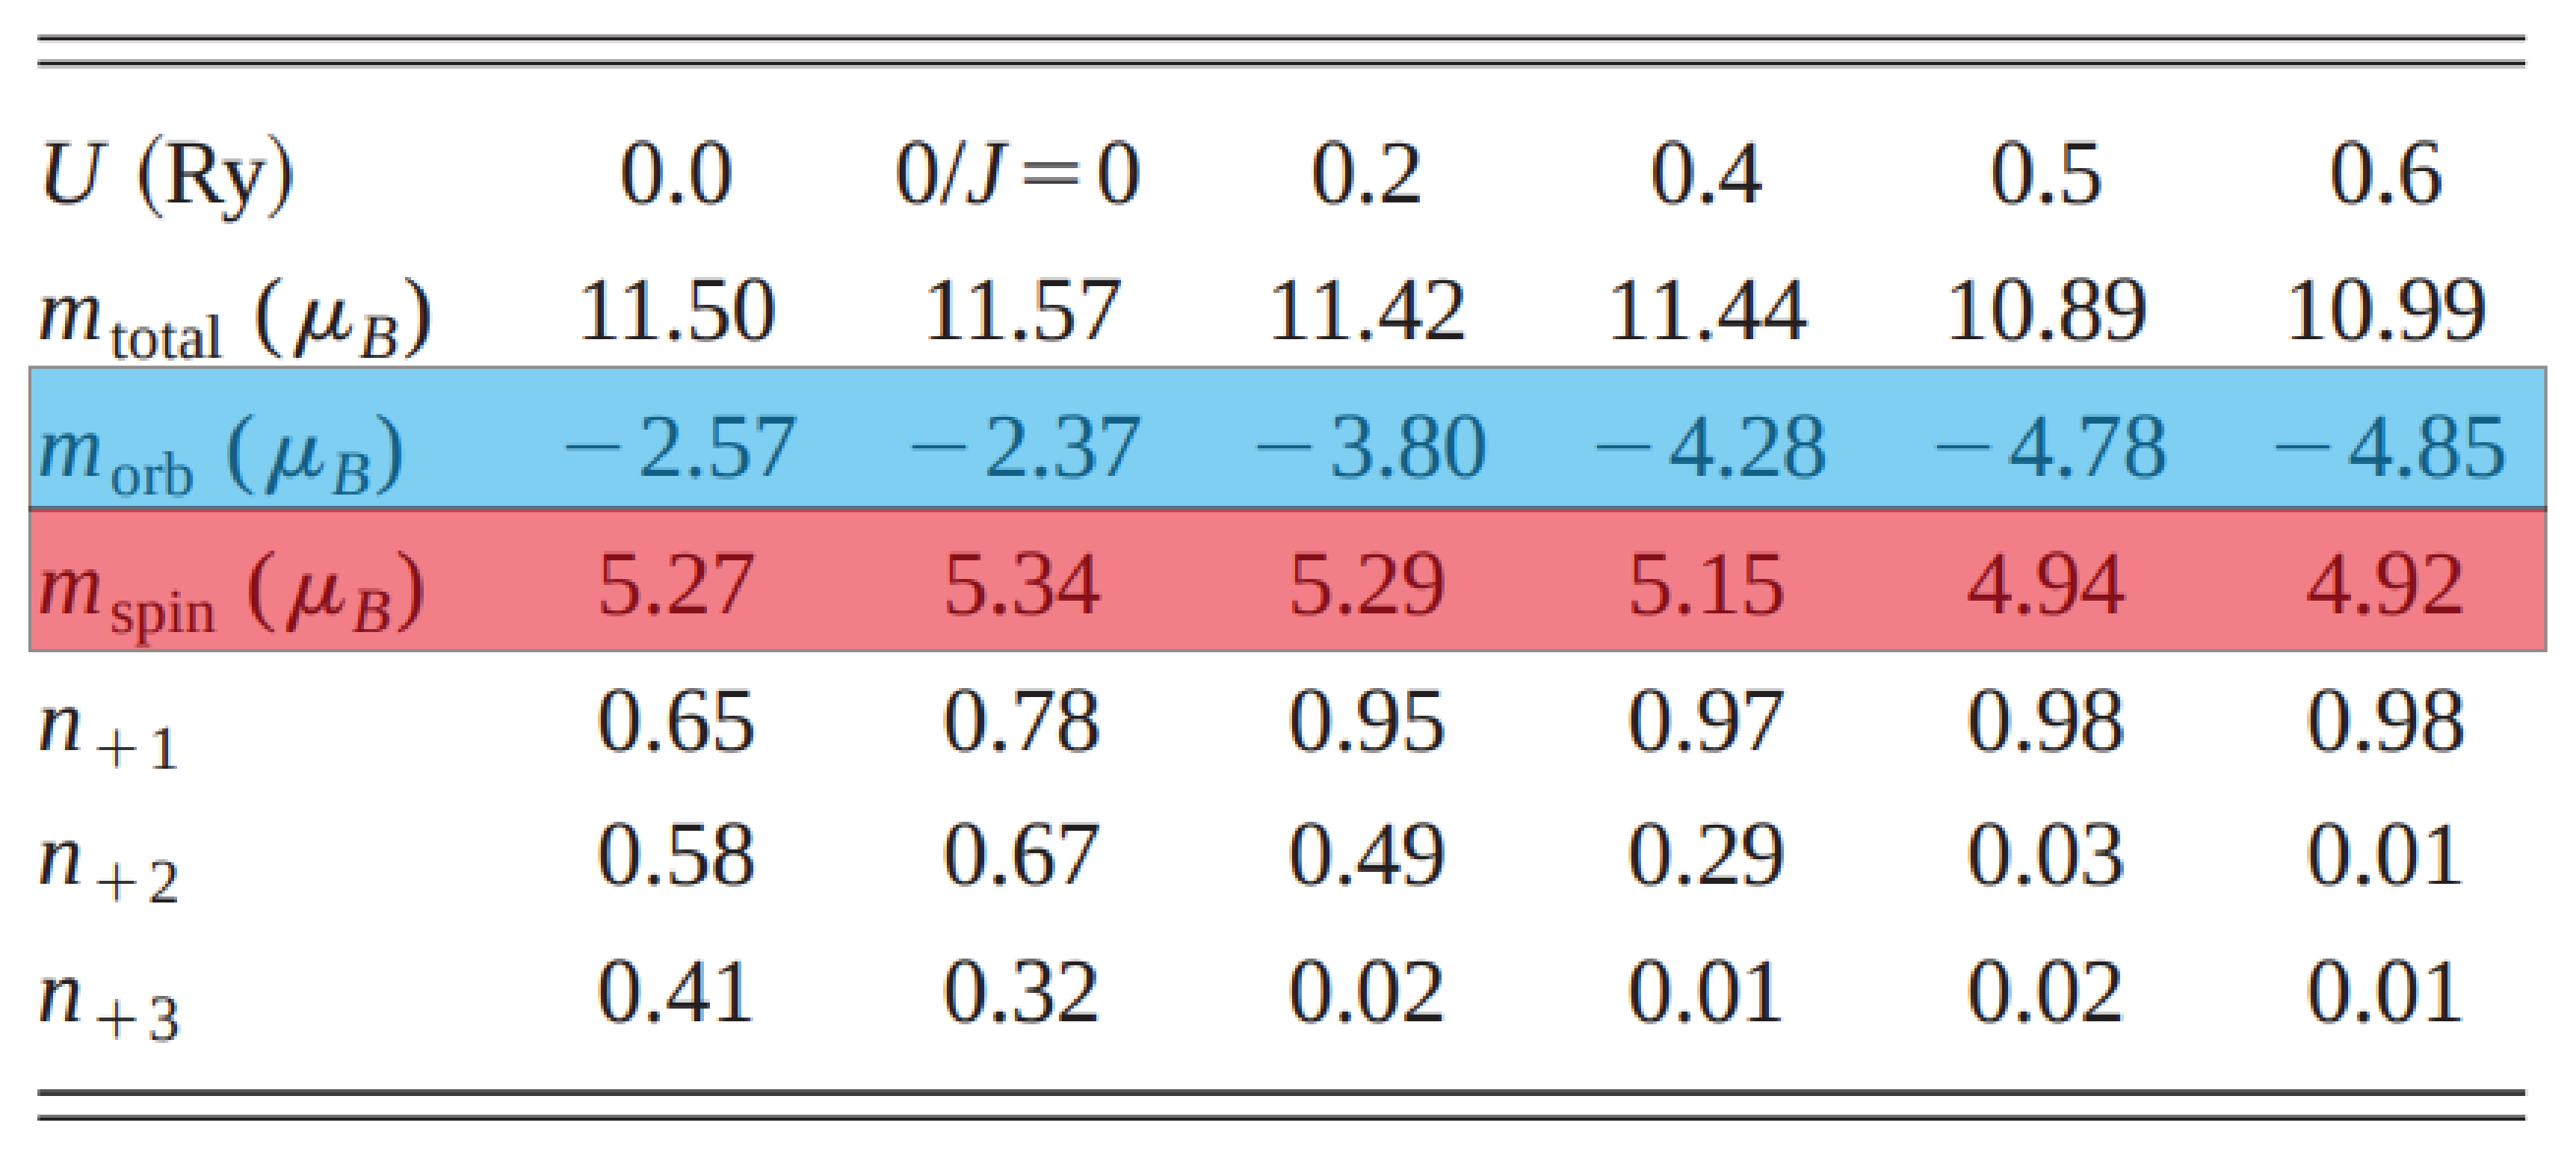
\includegraphics[width=\textwidth]{figure/SmAl2.png}
          \end{column}
          \begin{column}{0.6\textwidth}\footnotesize
            In this article, the DFT calculation result shows, the \textcolor{blue}{\(\bm{M}_{\text{orb}}\)} and \textcolor{red}{\(\bm{M}_{\text{spin}}\)} of Sm \(4f\) electrons in SmAl\(_2\) is comparable.
          \end{column}
        \end{columns}

        \item \purple{\href{https://doi.org/10.1103/PhysRevB.70.134418}{S. Qiao \emph{et al.}, Phys. Rev. B \textbf{70}, 134418 (2004).}}\\
        \begin{columns}
          \begin{column}{0.35\textwidth}
            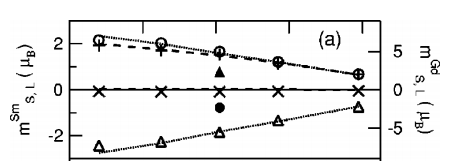
\includegraphics[width=\textwidth]{figure/SmGdAl2.png}
          \end{column}
          \begin{column}{0.6\textwidth}\footnotesize
            In this case, the x-ray experimental result shows that, the \(\bm{M}_{\text{spin}}\)(\(\bigcirc\)) and \(\bm{M}_{\text{orb}}\)(\(\triangle\)) of Sm in Sm\(_{0.982}\)Gd\(_{0.018}\)Al\(_2\) is equally contribute to the total magnetization, and therefore canceled with each other.
          \end{column}
        \end{columns}

        \item \purple{\href{https://doi.org/10.1103/PhysRevB.102.121406}{Si-Yu Li \emph{et al.}, Phys. Rev. B \textbf{102}, 121406(R) (2020).}}\\
        \begin{columns}
          \begin{column}{0.35\textwidth}
            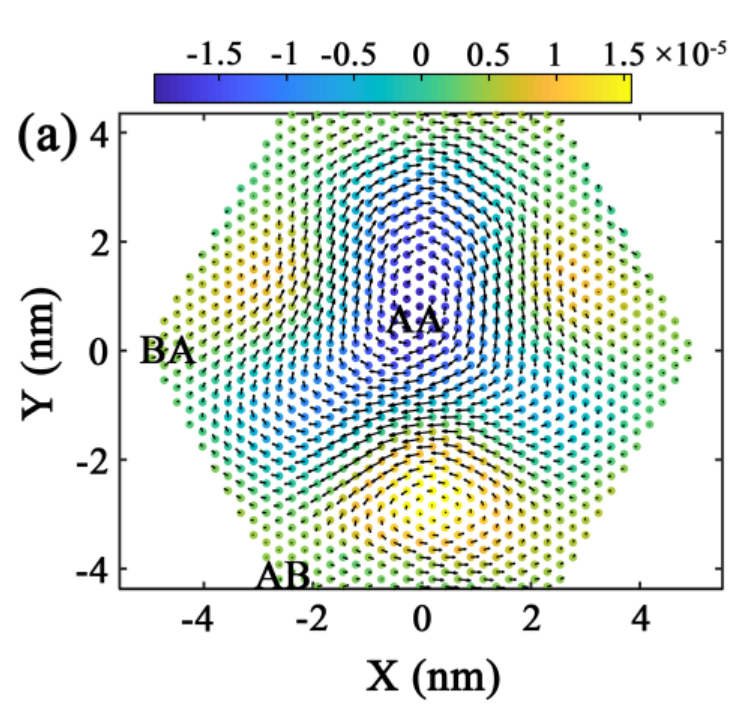
\includegraphics[width=0.75\textwidth]{figure/Graphene.png}
          \end{column}
          \begin{column}{0.6\textwidth}\footnotesize
            In twisted bilayer graphene, it is said that, the magnetization  mainly comes from the \(\bm{M}_{\text{orb}}\), which is about 10.7 \(\mu_B\) per moir\'e supercell.
          \end{column}
        \end{columns}
      \end{itemize}
    \end{frame}
    %-===================================================================-%
  
    \section{Attempt for Solving Orbital Magnetization}

    %+===================================================================+%
    \begin{frame}{From classical model to the quantum system}
      The classical defination of the magnetic moment is, 
      \begin{equation}
        \bm{m}_{\text{orb}} = \frac{1}{2c}\int\mathrm{d}^3r\;\bm{r}\times\bm{J} = \frac{1}{2c}\int\mathrm{d}^3r\;\bm{r}\times\rho\bm{v}
      \end{equation} 
      
      In the quantum system, the total orbital moment (\(\bm{m}_{\text{orb}}\)) is:
      \begin{subequations}\begin{align}
        \bm{m}_{\text{orb}} &= -\frac{e}{2c}\sum_n f_n \langle\psi_n|\widehat{\bm{r}}\times\widehat{\bm{v}}|\psi_n\rangle\\
        \bm{v} &= -\frac{i}{\hbar}[\widehat{\bm{r}}, \widehat{H}]
      \end{align}\end{subequations}

      Then, the orbital magnetization (\(\bm{M}_{\text{orb}}\)) can be defined as the magnetic moment per unit volume, 
      \begin{equation}
        \bm{M}_{\text{orb}} = \frac{\bm{m}_{\text{orb}}}{V_{\text{all}}} = -\frac{e}{2cV_{\text{all}}}\sum_n f_n \langle\psi_n|\widehat{\bm{r}}\times\widehat{\bm{v}}|\psi_n\rangle
      \end{equation}
      where the \purple{\(V_{\text{all}}\)} is the total volume of the target system.
    \end{frame}
    %-===================================================================-%

    %+===================================================================+%
    \begin{frame}{The ill-defined \(\widehat{\bm{r}}\) under Bloch states}\small
      In the solids, the eigenstates \(|\psi_n\rangle\) become Bloch states \(|\psi_{n\bm{k}}\rangle\) with the bloch wave vector \(\bm{k}\),
      \begin{subequations}
        \begin{align}
          \bm{M}_{\text{orb}} &= -\frac{e}{2cV_{\text{all}}}\sum_{n,\bm{k}} f_{n\bm{k}} \langle\psi_{n\bm{k}}|\widehat{\bm{r}}\times\widehat{\bm{v}}|\psi_{n\bm{k}}\rangle\\
          &= -\frac{e}{2c}\sum_{n}\int_{\text{BZ}}\frac{\mathrm{d}^dk}{(2\pi)^d} f_{n\bm{k}} \langle\psi_{n\bm{k}}|\widehat{\bm{r}}\times\widehat{\bm{v}}|\psi_{n\bm{k}}\rangle
        \end{align}
      \end{subequations}
      \begin{block}{}
        As we all know, the \(\widehat{\bm{r}}\) operator is ill-defined under Bloch states\footnote{\tiny \href{https://doi.org/10.1016/S0081-1947(08)60459-2}{E.I. Blount, Solid State Phys. \textbf{13}, 305 (1962).}},
      \begin{equation}\color{purple}
        \begin{aligned}
          \langle\psi_{n\bm{k}}|\widehat{\bm{r}}|\psi_{m\bm{k}'}\rangle &= (1-\delta_{nm})\delta(\bm{k}-\bm{k}')\bm{A}_{nm}(\bm{k}) \\
          &+ \delta_{nm}\left[\delta(\bm{k}-\bm{k}')\bm{A}_{nn} + i\dfrac{\partial}{\partial \bm{k}}\delta(\bm{k}-\bm{k}')\right]
        \end{aligned}
      \end{equation}
      where, \purple{\(\bm{A}\)} is Berry connection, which is gauge dependent. Thus, \purple{\(\langle\psi_{n\bm{k}}|\widehat{\bm{r}}|\psi_{n\bm{k}}\rangle\)} is divergent. 
      \end{block}
    \end{frame}
    %-===================================================================-%

    %+===================================================================+%
    \begin{frame}{Using local bulk current?}
      One may hope to solve the problem from the point of view of local bulk current density \(\bm{J}(\bm{r})\).
      
      \begin{columns}
        \begin{column}{0.3\textwidth}
          \textcolor{white}{.}
          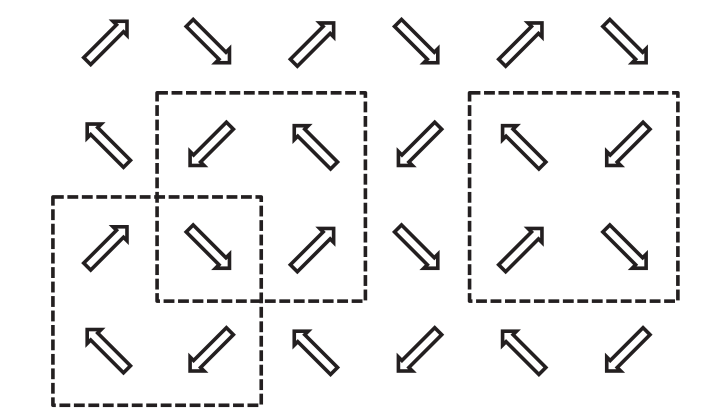
\includegraphics[width=\textwidth]{figure/MinJ.png}
        \end{column}
        \begin{column}{0.7\textwidth}    
          \begin{block}{}
            But in fact, the knowledge of \(\bm{J}(\bm{r})\), in principle, is insufficient to calculate the \(\bm{M}_{\text{orb}}\). \textcolor{gray}{Just like what happend when we try to using the electron density \(\rho(\bm{r})\) to get the electric polarization \(\bm{P}\) in solids.}
          \end{block}
        \end{column}
      \end{columns}
      \ \\
     
      To see this, we define the magnetization \(\bm{\mathcal{M}}_{\text{orb}}(\bm{r})\) via \(\bm{J}(\bm{r})\), 
      \begin{equation}
        c\nabla\times\bm{\mathcal{M}}_{\text{orb}}(\bm{r}) = \bm{J}(\bm{r})
      \end{equation}

      However, \(\bm{\mathcal{M}}_{\text{orb}}(\bm{r})\) can simply be repalced by another \(\bm{\mathcal{M}}'_{\text{orb}}(\bm{r})\), which corresponding to the same \(\bm{J}(\bm{r})\),
      \begin{equation}
        \bm{\mathcal{M}}_{\text{orb}}(\bm{r}) \to \bm{\mathcal{M}}'_{\text{orb}}(\bm{r}) = \bm{\mathcal{M}}_{\text{orb}}(\bm{r}) + \bm{\mathcal{M}}_{\text{orb}}^0 + \nabla\xi(\bm{r})
      \end{equation}
    \end{frame}
    %-===================================================================-%

    %+===================================================================+%
    \begin{frame}{Muffin-tin approximation}
      \begin{columns}
        \begin{column}{0.27\textwidth}
          \begin{center}
            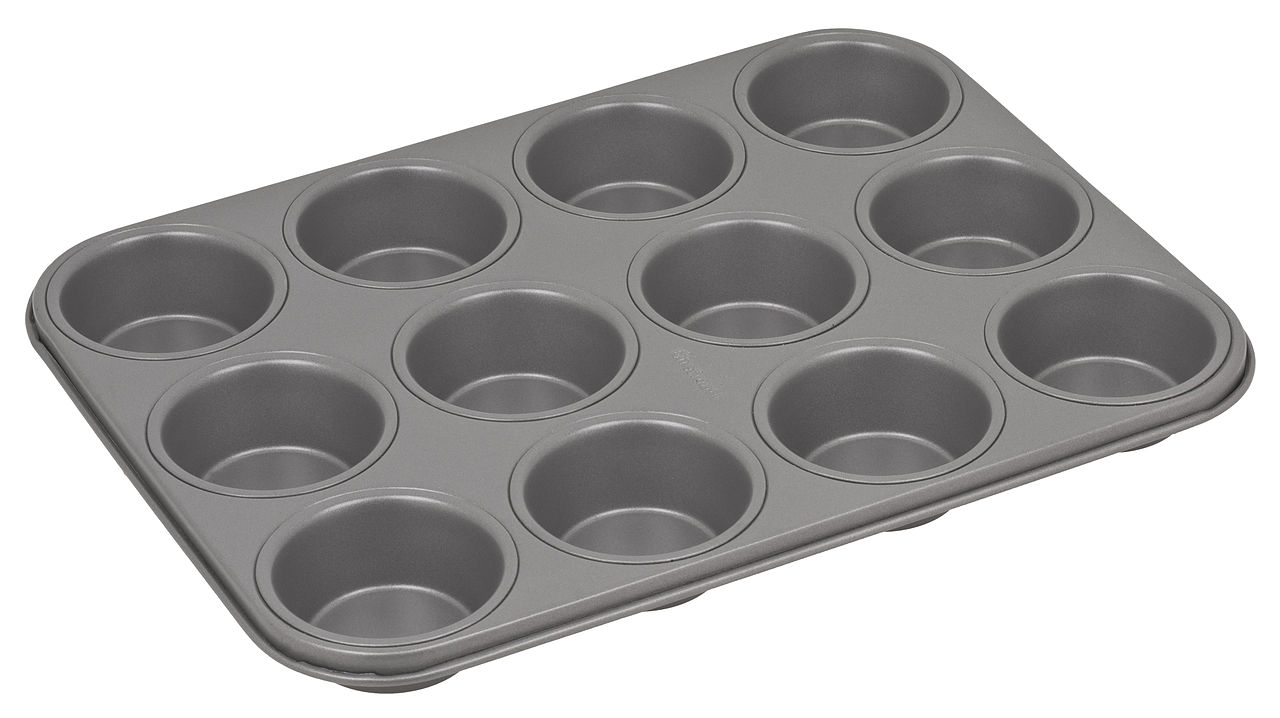
\includegraphics[width=\textwidth]{figure/muffin-tin.jpg}
          \end{center}
        \end{column}
        \begin{column}{0.7\textwidth}
        \begin{block}{}
          Non-overlapping muffin-tin spheres center around the atoms in solids. Within these spheres, which are finite systems, the moment can be calculated accroding to, 
          \begin{equation}
            \bm{m}_{\text{orb}} = -\frac{e}{2c}\sum_{n\bm{k}} f_n \langle\psi_{n\bm{k}}|\widehat{\bm{r}}\times\widehat{\bm{v}}|\psi_{n\bm{k}}\rangle
          \end{equation}
        \end{block}
        \end{column}
      \end{columns}
      \ \\
      
      Often, the orbital magnetization indeed originates from regions near the atom cores, making this approximation acceptable.
      
      \begin{table}\scriptsize
        \caption{\scriptsize Orbital magnetization using muffin-tin approximation\footnote{\tiny \href{https://doi.org/10.1142/S0217979211058912}{T. Thonhauser, Int. J. Mod. Phys. B \textbf{25}, 1429 (2011).}} (in \(\mu_B\))}
        \begin{tabular}{c|ccccc}
          \toprule
          Material & \(\bm{M}_{\text{orb}}^{\text{Exp}}\) & \(\bm{M}_{\text{orb}}^{\text{DFT}}\) & muffin-tin & interstitial\\
          \midrule
          \(bcc\) - Fe & 0.081 & 0.066 & 0.043 & 0.023\\
          \(fcc\) - Co & 0.120 & 0.076 & 0.063 & 0.013\\
          \(fcc\) - Ni & 0.053 & 0.052 & 0.051 & 0.001\\
          \bottomrule
        \end{tabular}
      \end{table}
    \end{frame}
    %-===================================================================-%

    \section{Modern Theory of Orbital Magnetization}

    %+===================================================================+%
    \begin{frame}{Derivation in the Wannier representation}
      \small
      For now, let us focus on a simplest model: a \purple{2D finite but large enough} solid, with \purple{one topological  trivial insulating band}, described by \purple{spinless} Hamiltonlian with \purple{broken time-reversal symmetry}. As we show above, its orbital magnetization can be expressed as,
      \begin{equation}
        \bm{M}_{\text{orb}} = -\frac{e}{2cV_{\text{all}}}\sum_{\bm{k}} \langle\psi_{\bm{k}}|\widehat{\bm{r}}\times\widehat{\bm{v}}|\psi_{\bm{k}}\rangle
      \end{equation}

      Using the Wannier representation, 
      \begin{equation}
        \label{eq::Morb_wannier}
        \bm{M}_{\text{orb}} = -\frac{e}{2cV_{\text{all}}}\sum_{\bm{R}} \langle\omega_{\bm{R}}|\widehat{\bm{r}}\times\widehat{\bm{v}}|\omega_{\bm{R}}\rangle
      \end{equation}
      where \purple{\(\bm{R}\)} traverses all primitive cells in the solid.
      \begin{block}{Key Point}
        It must be noted that, the Wannier function in such a solid system can be split into two regions: ``\purple{in the bulk}'' and ``\purple{on the surface}''. Those two regions behave totally differently when it comes to Eq. \eqref{eq::Morb_wannier}.
      \end{block}
    \end{frame}
    %-===================================================================-%  

    %+===================================================================+%
    \begin{frame}{Two terms in orbital magnetization}\small
      \begin{equation}\begin{aligned}
        \bm{M}_{\text{orb}} &= -\frac{e}{2cV_{\text{all}}}\sum_{\bm{R}}^{\text{all}} \langle\omega_{\bm{R}}|\widehat{\bm{r}}\times\widehat{\bm{v}}|\omega_{\bm{R}}\rangle\\
        &\;{\color{gray}= -\frac{e}{2cV_{\text{all}}}\sum_{\bm{R}}^{\text{bulk}}\langle\omega_{\bm{R}}|\widehat{\bm{r}}\times\widehat{\bm{v}}|\omega_{\bm{R}}\rangle 
        -\frac{e}{2cV_{\text{all}}}\sum_{\bm{R}}^{\text{surf}}\langle\omega_{\bm{R}}|\widehat{\bm{r}}\times\widehat{\bm{v}}|\omega_{\bm{R}}\rangle} \\
        &= -\frac{e}{2cV_{\text{all}}}\sum_{\bm{R}}^{\text{all}} \langle\omega_{\bm{R}}|\left(\widehat{\bm{r}}-\bm{r}_{\bm{R}}\right)\times\widehat{\bm{v}}|\omega_{\bm{R}}\rangle
        -\frac{e}{2cV_{\text{all}}}\sum_{\bm{R}}^{\text{all}} \langle\omega_{\bm{R}}|\bm{r}_{\bm{R}}\times\widehat{\bm{v}}|\omega_{\bm{R}}\rangle\\
        &= \bm{M}_{\text{orb}}^{\text{LC}} + \bm{M}_{\text{orb}}^{\text{IC}}
      \end{aligned}\end{equation}
      where \(\mathcal{O}_s = \langle\omega_s|\widehat{\mathcal{O}}|\omega_s\rangle\).
      \begin{columns}
        \begin{column}{0.3\textwidth}
          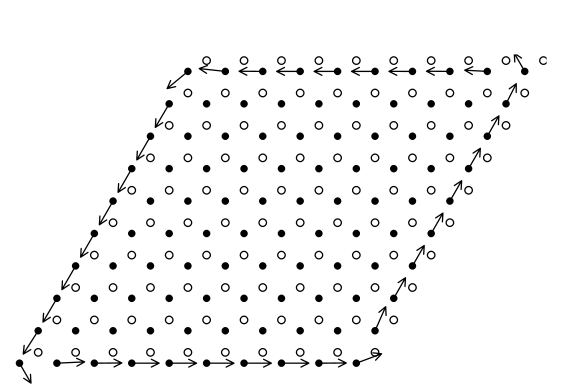
\includegraphics[width=\textwidth]{figure/edge-solid.png}
        \end{column}
        \begin{column}{0.7\textwidth}
          \begin{block}{}
            The 1st term is what we called ``\purple{local circulation(LC)}'' term, the 2nd is ``\purple{itinerant circulation(IC)}''. And, as what we show in second step, the \(\bm{R}\) summation contants the \purple{bulk} and \purple{surface} regions. 
          \end{block}
        \end{column}
      \end{columns}
    \end{frame}
    %-===================================================================-%  

    %+===================================================================+%
    \begin{frame}[fragile,t]{Local circulation term \(\bm{M}_{\text{orb}}^{\text{LC}}\)}\scriptsize
      \begin{columns}
        \begin{column}{0.3\textwidth}
          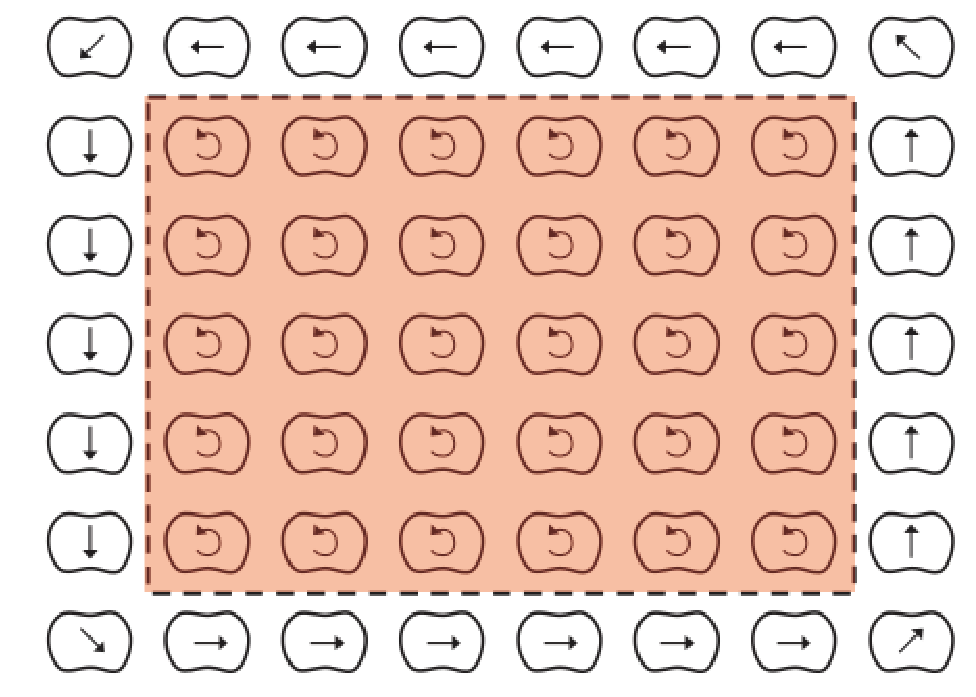
\includegraphics[width=\textwidth]{figure/edge-solid2-bulk.png}
        \end{column}
        \begin{column}{0.5\textwidth}
          \begin{block}{}
            The ``LC'' term corresponding to the magnetization mainly generated by the bulk electrons.
          \end{block}
        \end{column}
      \end{columns}
      \begin{equation}\begin{aligned}
        \bm{M}_{\text{orb}}^{\text{LC}} &= -\frac{e}{2cV_{\text{all}}}\sum_{\bm{R}}^{\text{all}} \langle\omega_{\bm{R}}|\left(\widehat{\bm{r}}-\bm{r}_{\bm{R}}\right)\times\widehat{\bm{v}}|\omega_{\bm{R}}\rangle\\
        &\approx -\frac{e}{2cV_{\text{all}}}\sum_{\bm{R}}^{\text{bulk}} \langle\omega_{\bm{R}}|\left(\widehat{\bm{r}}-\bm{r}_{\bm{R}}\right)\times\widehat{\bm{v}}|\omega_{\bm{R}}\rangle\\
        &= -\frac{e}{2cV_{\text{all}}}(N-n)\langle\omega_{\bm{0}}|\left(\widehat{\bm{r}}-\bm{r}_{\bm{0}}\right)\times\widehat{\bm{v}}|\omega_{\bm{0}}\rangle\\
        &\approx -\frac{eN}{2cV_{\text{all}}}\langle\omega_{\bm{0}}|\left(\widehat{\bm{r}}-\bm{r}_{\bm{0}}\right)\times\widehat{\bm{v}}|\omega_{\bm{0}}\rangle\\
        &= -\frac{e}{2cV_{\text{cell}}}\langle\omega_{\bm{0}}|\widehat{\bm{r}}\times\widehat{\bm{v}}|\omega_{\bm{0}}\rangle
      \end{aligned}\end{equation}
      {\scriptsize where the \purple{\(n\)} and \purple{\(N\)} is the Wannier functions' quantity on the surface and in the whole system, while \(N \sim n^2\).  \purple{\(\omega_{\bm{0}}\)} is one Wannier function in the bulk, \purple{\(V_{\text{cell}}\)} is the volume of a primitive cell.}
    \end{frame}
    %-===================================================================-%   

    %+===================================================================+%
    \begin{frame}[fragile,t]{Itinerant circulation term \(\bm{M}_{\text{orb}}^{\text{IC}}\)}
      \scriptsize
      \begin{columns}
        \begin{column}{0.3\textwidth}
          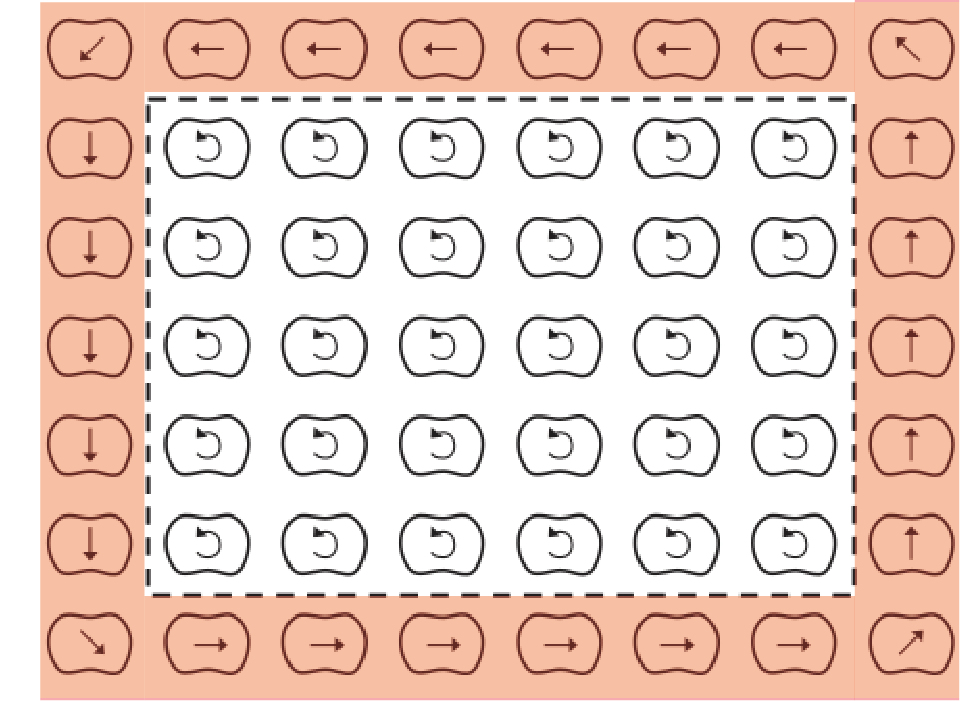
\includegraphics[width=\textwidth]{figure/edge-solid2-edge.png}
        \end{column}
        \begin{column}{0.5\textwidth}
          \begin{block}{}
            The ``IC'' term corresponding to the magnetization mainly generated by the surface electrons.
          \end{block}
        \end{column}
      \end{columns}
      \begin{equation}\begin{aligned}
        \bm{M}_{\text{orb}}^{\text{IC}} &= -\frac{e}{2cV_{\text{all}}}\sum_{\bm{R}}^{\text{all}} \langle\omega_{\bm{R}}|\bm{r}_{\bm{R}}\times\widehat{\bm{v}}|\omega_{\bm{R}}\rangle\\
        &= -\frac{e}{2cV_{\text{all}}}\sum_{\bm{R}}^{\text{all}} \bm{r}_{\bm{R}}\times\bm{v}_{\bm{R}}\\
        &= -\frac{e}{2cV_{\text{all}}}\sum_{\bm{R}}^{\text{surf}} \bm{r}_{\bm{R}}\times\bm{v}_{\bm{R}}\\
        & \;{\color{gray}\approx -\frac{e}{2cV_{\text{cell}}} \frac{n}{N}\bm{r}_{\text{surf}}\times\bm{v}_{\text{surf}}}
      \end{aligned}\end{equation}
      where, \purple{\(\bm{r}_{\text{surf}}\)} and \purple{\(\bm{v}_{\text{surf}}\)} is the absolute position and velocity of the surface wannier functions.
    \end{frame}
    %-===================================================================-%
    
    %+===================================================================+%
    \begin{frame}{Express \(\bm{M}_{\text{orb}}^{\text{IC}}\) using bulk Wannier functions (2D system)}
      \scriptsize
      With some tricky derivation\footnote{\tiny \href{https://doi.org/10.1103/PhysRevLett.95.137205}{T. Thonhauser \emph{et al.}, Phys. Rev. Lett. \textbf{95}, 137205 (2005).}}, one can express the \(\bm{M}_{\text{orb}}^{\text{IC}}\) with bulk Wannier functions.
      \begin{equation}\begin{aligned}
        M_{\text{orb}}^{\text{IC}, z} &= -\frac{e}{2cV_{\text{all}}}\sum_{\bm{R}}^{\text{surf}} \bm{r}_{\bm{R}}\times\bm{v}_{\bm{R}}\\
        &= \frac{e}{2\hbar{}cV_{\text{cell}}}\text{Im}\left\{\sum_{\bm{R}} \langle\omega_{\bm{0}}|\widehat{H}|\omega_{\bm{R}}\rangle\left(R_x\langle\omega_{\bm{R}}|\widehat{y}|\omega_{\bm{0}}\rangle - R_y\langle\omega_{\bm{R}}|\widehat{x}|\omega_{\bm{0}}\rangle\right)\right\}
      \end{aligned}\end{equation}
      where, \purple{\(\widehat{\bm{r}} = (\widehat{x}, \widehat{y}, \widehat{z})\)}, \purple{\(\bm{R} = (R_x, R_y, R_z)\)}, \purple{\(M_{\text{orb}}^{\text{IC}, z}\)} represent the magnetization in \(z\) direction, for this is a 2D system.
     
      \begin{columns}
        \begin{column}{0.3\textwidth}
          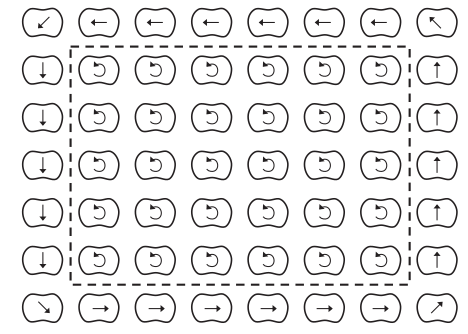
\includegraphics[width=\textwidth]{figure/edge-solid2.png}
        \end{column}
        \begin{column}{0.6\textwidth}
          \begin{alertblock}{}
            \purple{BE CAREFUL}, the relation above is valid only when the edge states \purple{can merge into the bulk adiabatically}.
          \end{alertblock}
          \begin{block}{}
            The surface term can express with the bulk wannier functions.
          \end{block}
        \end{column}
      \end{columns}
    \end{frame}
    %-===================================================================-%

    %+===================================================================+%
    \begin{frame}{Back to Bloch representation (2D system)}
      The final step is transform the expressions for \(\bm{M}_{\text{orb}}^{\text{LC}}\) and \(\bm{M}_{\text{orb}}^{\text{IC}}\)back to the Bloch representation. 
      \begin{subequations}\begin{align}
        |\omega_{\bm{R}}\rangle &= \frac{V_{\text{cell}}}{(2\pi)^d}\int\mathrm{d}^dk\; \mathrm{e}^{-i\bm{k}\cdot(\bm{r}-\bm{R})}|u_{\bm{k}}\rangle\\
        |u_{\bm{k}}\rangle &= \mathrm{e}^{-i\bm{k}\cdot\bm{r}}|\psi_{\bm{k}}\rangle
      \end{align}\end{subequations}
      Little surprisingly, we get quite a concise formula,
      \begin{subequations}\begin{align}
        M_{\text{orb}}^{\text{LC}, z} &= \frac{e}{\hbar{}c}\text{Im}\int_{\text{BZ}}\frac{\mathrm{d}^2k}{(2\pi)^2}\langle\partial_xu_{\bm{k}}|\widehat{H}_{\bm{k}}|\partial_yu_{\bm{k}}\rangle\\
        M_{\text{orb}}^{\text{IC}, z} &= \frac{e}{\hbar{}c}\text{Im}\int_{\text{BZ}}\frac{\mathrm{d}^2k}{(2\pi)^2}\langle\partial_xu_{\bm{k}}|E_{\bm{k}}|\partial_yu_{\bm{k}}\rangle
      \end{align}\end{subequations}
      where, \purple{\(\partial_i \equiv \partial/\partial{}k_i\)}, \purple{\(\widehat{H}_{\bm{k}} \equiv \mathrm{e}^{-i\bm{k}\cdot\bm{r}}\widehat{H}\mathrm{e}^{i\bm{k}\cdot\bm{r}}\)}, the \purple{\(E_{\bm{k}}\)} denote the corresponding eigenvalues.
    \end{frame}
    %-===================================================================-% 

    %+===================================================================+%
    \begin{frame}{Extended to 3D}
      The oribtal magnetization formula can be easily extended to 3D, 
      \begin{subequations}\begin{align}
        \bm{M}_{\text{orb}}^{\text{LC}} &= \frac{e}{2\hbar{}c}\text{Im}\int_{\text{BZ}}\frac{\mathrm{d}^3k}{(2\pi)^3}\langle\nabla_{\bm{k}}u_{\bm{k}}|\times\widehat{H}_{\bm{k}}|\nabla_{\bm{k}}u_{\bm{k}}\rangle\\
        \bm{M}_{\text{orb}}^{\text{IC}} &= \frac{e}{2\hbar{}c}\text{Im}\int_{\text{BZ}}\frac{\mathrm{d}^3k}{(2\pi)^3}\langle\nabla_{\bm{k}}u_{\bm{k}}|\times{}E_{\bm{k}}|\nabla_{\bm{k}}u_{\bm{k}}\rangle
      \end{align}\end{subequations}
      
      You may already notice that, the ``IC'' term can further be written with the Berry curvature \(\bm{\Omega}_{\bm{k}}\), 
      \begin{equation}
        \bm{M}_{\text{orb}}^{\text{IC}} = -\frac{e}{2\hbar{}c}\int_{\text{BZ}}\frac{\mathrm{d}^3k}{(2\pi)^3}E_{\bm{k}}\bm{\Omega}_{\bm{k}}
      \end{equation}
      Anyway, for now, we get the orbital magnetization for a one band spinless trivial insulating system, 
      \begin{block}{}
        \begin{equation}
          \bm{M}_{\text{orb}} = \frac{e}{2\hbar{}c}\text{Im}\int_{\text{BZ}}\frac{\mathrm{d}^3k}{(2\pi)^3}\langle\nabla_{\bm{k}}u_{\bm{k}}|\times(\widehat{H}_{\bm{k}}+E_{\bm{k}})|\nabla_{\bm{k}}u_{\bm{k}}\rangle
        \end{equation}
      \end{block}
    \end{frame}
    %-===================================================================-% 

    %+===================================================================+%
    \begin{frame}{A paradox about the energy shift}\small
      As we all know, an energy shift on the Hamiltonlian does not change its physical behaviors, but
      \begin{equation}
        \begin{aligned}
          \bm{M}_{\text{orb}}\to\bm{M}_{\text{orb}}' &= \frac{e}{2\hbar{}c}\text{Im}\int_{\text{BZ}}\frac{\mathrm{d}^3k}{(2\pi)^3}\langle\nabla_{\bm{k}}u_{\bm{k}}|\times(\widehat{H}_{\bm{k}}+\varepsilon+E_{\bm{k}}+\varepsilon)|\nabla_{\bm{k}}u_{\bm{k}}\rangle\\
          \Delta\bm{M}_{\text{orb}} &= \bm{M}_{\text{orb}}'-\bm{M}_{\text{orb}} = \frac{e\varepsilon}{\hbar{}c(2\pi)^2}\bm{C}
        \end{aligned}
      \end{equation}
      where, \purple{\(\bm{C} = (C_x, C_y, C_z)\)} is the Chern number in three directions, \purple{\(\varepsilon\)} is the energy shift of the Hamiltonlian.

      \begin{alertblock}{Paradox}
        That means, in a system whose Chern number not equal to zero (e.g., metal or topological non-trivial insulator), there will be something weird.
      \end{alertblock}

      \begin{block}{}
        The explanation for this ``paradox'' can be revealed from the pre-condition that the following equation satisfied.
        \begin{equation*}
          \bm{M}_{\text{orb}}^{\text{IC}} = \frac{e}{2\hbar{}c}\text{Im}\int_{\text{BZ}}\frac{\mathrm{d}^3k}{(2\pi)^3}\langle\nabla_{\bm{k}}u_{\bm{k}}|\times{}E_{\bm{k}}|\nabla_{\bm{k}}u_{\bm{k}}\rangle
        \end{equation*}
      \end{block}
    \end{frame}
    %-===================================================================-% 

    %+===================================================================+%
    \begin{frame}{Orbital magnetization for non-zero Chern number system}
      \begin{block}{}
        \begin{equation*}
          \bm{M}_{\text{orb}}^{\text{IC}} \overset{\circ}{=} \frac{e}{2\hbar{}c}\text{Im}\int_{\text{BZ}}\frac{\mathrm{d}^3k}{(2\pi)^3}\langle\nabla_{\bm{k}}u_{\bm{k}}|\times{}E_{\bm{k}}|\nabla_{\bm{k}}u_{\bm{k}}\rangle
        \end{equation*}
        As we mention before, there is a pre-condition (\(\circ\)) when we using the bulk wannier function represent ``IC'' term, that is, \purple{the edge states can merge into the bulk adiabatically}. But for the edge states protected by the topology, obviously, that pre-condition cannot be satisfied.
      \end{block}
      \begin{block}{Topological edge states term}
        In other words, the \(\bm{M}_{\text{orb}}\) must add a 3rd term corresponding to the topological edge state. Let us show it first and explain later.
        \begin{equation}
          \bm{M}_{\text{orb}}^{\text{TP}} = \frac{e}{2\hbar{}c}\text{Im}\int_{\text{BZ}}\frac{\mathrm{d}^3k}{(2\pi)^3}\langle\nabla_{\bm{k}}u_{\bm{k}}|\times(-2\mu_{0})|\nabla_{\bm{k}}u_{\bm{k}}\rangle
        \end{equation}
        where, \purple{\(\mu_{0}\)} is the chemical potential under zero temperature, which is exzactly the Fermi energy, \purple{\(\mu_{0} = E_{\text{F}}\)}.
      \end{block}
    \end{frame}
    %-===================================================================-% 

    %+===================================================================+%
    \begin{frame}{Topological edge states term}\scriptsize
      Now, let us consider a 2D system,
      \begin{equation}
        M_{\text{orb}}^{\text{TP},z} = \frac{e}{\hbar{}c}\text{Im}\int_{\text{BZ}}\frac{\mathrm{d}^2k}{(2\pi)^2}\langle\partial_xu_{\bm{k}}|(-2\mu_{0})|\partial_yu_{\bm{k}}\rangle
      \end{equation}
      \begin{equation}
        \label{eq::mzorb}
        \frac{\mathrm{d}M_{\text{orb}}^z}{\mathrm{d}\mu_{0}} = \frac{\mathrm{d}M_{\text{orb}}^{\text{TP},z}}{\mathrm{d}\mu_{0}} = -\frac{e}{2\pi\hbar{}c}C
      \end{equation}
      Owing to the main equation \(c\nabla\times\bm{M} = \bm{j}\), a macroscopic current of intensity \(I = cM_{\text{orb}}^z\), together with Eq. \eqref{eq::mzorb}, 
      \begin{equation}
        \label{eq::c1}
        \frac{\mathrm{d}I}{\mathrm{d}\mu_{0}} = -\frac{eC}{2\pi\hbar}
      \end{equation}
      \begin{columns}
        \begin{column}{0.25\textwidth}
          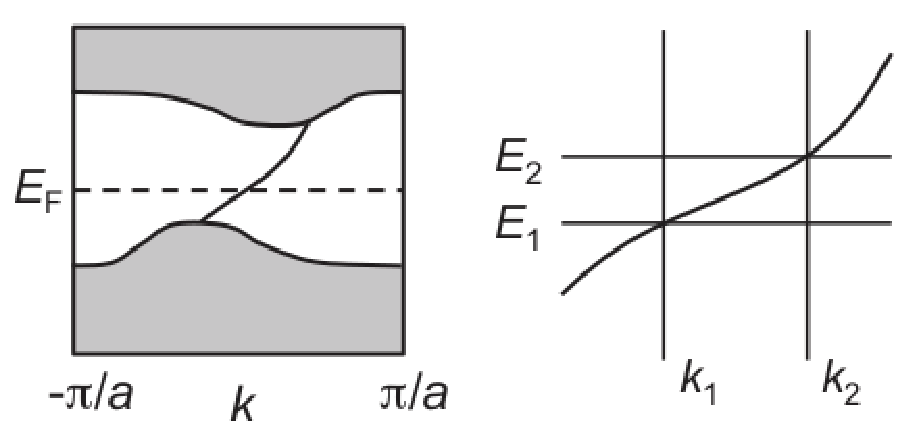
\includegraphics[width=\textwidth]{figure/Ef-velocity.png}
        \end{column}
        \begin{column}{0.75\textwidth}
          On the other hand, raising the chemical potential by \purple{\(\mathrm{d}\mu_{0}\)} fills \purple{\(\mathrm{d}k/2\pi\)} states per unit length on one band, which means,
      \begin{equation}
        \label{eq::c2}
        \mathrm{d}I = -env\frac{\mathrm{d}k}{2\pi} = -en\frac{1}{\hbar}\frac{\mathrm{d}E_\text{total}}{\mathrm{d}k}\frac{\mathrm{d}k}{2\pi} \approx -\frac{en}{2\pi\hbar}\mathrm{d}\mu_0
      \end{equation}
      where, \purple{\(v\)} is the electrons' group velocity, \purple{\(n\)} is the bands' quantity that participate in conducting.
        \end{column}
      \end{columns}
    
      \begin{block}{}
        Compare Eq. \eqref{eq::c1} and Eq. \eqref{eq::c2}, we can conclude that, \purple{the Chern number \(C\) is exzactly the number of chiral edge channels \(n\).}
      \end{block}
    \end{frame}
    %-===================================================================-% 

    %+===================================================================+%
    \begin{frame}{Final formula for orbital magnetization in solids}\small
      \begin{block}{Orbital Magnetization}
        \begin{subequations}\begin{align}
          \bm{M}_{\text{orb}} &= \frac{e}{2\hbar{}c}\text{Im}\int_{\text{BZ}}\frac{\mathrm{d}^3k}{(2\pi)^3}\langle\nabla_{\bm{k}}u_{\bm{k}}|\times(\widehat{H}_{\bm{k}}+E_{\bm{k}}-2\mu_{0})|\nabla_{\bm{k}}u_{\bm{k}}\rangle\\
          &= \frac{e}{2\hbar{}c}\text{Im}\int_{\text{BZ}}\frac{\mathrm{d}^3k}{(2\pi)^3}\langle\nabla_{\bm{k}}u_{\bm{k}}|\times(\widehat{H}_{\bm{k}}+E_{\bm{k}}-2E_{\text{F}})|\nabla_{\bm{k}}u_{\bm{k}}\rangle
        \end{align}\end{subequations}
      \end{block}
    \end{frame}
    %-===================================================================-% 

    %+===================================================================+%
    \begin{frame}{Orbital Magnetization for Multiple Bands}\small
      For the multiple band case, we just need to include the summation for bands,
      \begin{block}{Orbital Magnetization for Multiple Bands}
        \begin{subequations}\begin{align}
          \bm{M}_{\text{orb}} &= \frac{e}{2\hbar{}c}\text{Im}\sum_n\int_{\text{BZ}}\frac{\mathrm{d}^3k}{(2\pi)^3}f_{n\bm{k}}\langle\nabla_{\bm{k}}u_{n\bm{k}}|\times(\widehat{H}_{\bm{k}}+E_{n\bm{k}}-2\mu_{0})|\nabla_{\bm{k}}u_{n\bm{k}}\rangle\\
          &= \frac{e}{2\hbar{}c}\text{Im}\sum_n\int_{\text{BZ}}\frac{\mathrm{d}^3k}{(2\pi)^3}f_{n\bm{k}}\langle\nabla_{\bm{k}}u_{n\bm{k}}|\times(\widehat{H}_{\bm{k}}+E_{n\bm{k}}-2E_{\text{F}})|\nabla_{\bm{k}}u_{n\bm{k}}\rangle
        \end{align}\end{subequations}
        where, \purple{\(f_{n\bm{k}}\)} is the electrons occupation function.
      \end{block}
    \end{frame}
    %-===================================================================-% 

    %+===================================================================+%
    \begin{frame}{The semi-classical derivation for \(\bm{M}_{\text{orb}}\)  (Part I)}\small
      \begin{tcolorbox}[beamer,width=\textwidth,arc=0pt,boxsep=0.3pt,left=0pt,right=0pt,top=0pt,bottom=0pt]
        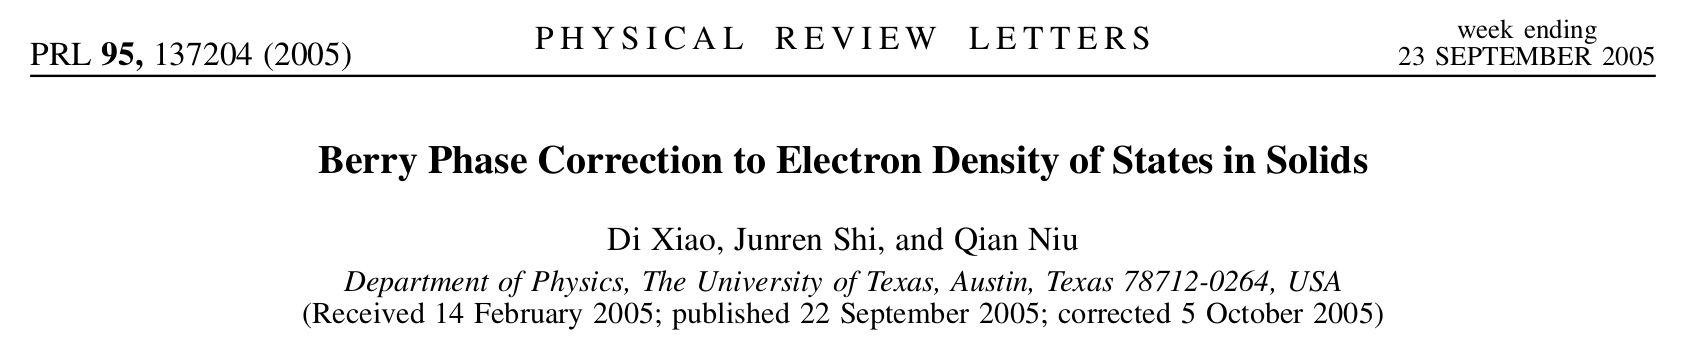
\includegraphics[width=\textwidth]{figure/classical-Morb.png}
      \end{tcolorbox}
      \ \\

      A very different derivation of \(\bm{M}_{\text{orb}}\) was given by Di Xiao \emph{et al.} based on the semiclassical theory, 
      \begin{subequations}
        \label{eq::niuq}\scriptsize
        \begin{align}
          \dot{\bm{r}} &= \frac{1}{\hbar}\partial_{\bm{k}}E_{n}(\bm{k}) - \dot{\bm{k}}\times\bm{\Omega}_{n}(\bm{k})\\
          \dot{\bm{k}} &= -\frac{e}{\hbar}\bm{F}(\bm{r}) - \frac{e}{\hbar}\dot{\bm{r}}\times\bm{B}(\bm{r})\\
          {\color{purple}n_e }&\;{\color{purple}= \frac{N_e}{V_{\text{all}}} = \int^{\mu(\bm{B})}\frac{\mathrm{d}^dk}{(2\pi)^d}\left(1 + \frac{e\bm{B}\cdot\bm{\Omega}}{\hbar}\right)}
        \end{align}
      \end{subequations}
      In 1999, Sundaram and Niu observed that, the orbital magnetic moment of a wave packet centered at \(\bm{k}\) in band \(n\) is,\footnote{\tiny \href{https://doi.org/10.1103/PhysRevB.59.14915}{G. Sundaram \emph{et al.}, Phys. Rev. B \textbf{59}, 14915 (1999).}}
      \begin{equation}
        \label{eq::xiaodi}
        \bm{m}_{n\bm{k}} = \frac{-ie}{2\hbar{}c}\langle\nabla_{\bm{k}}u_{n\bm{k}}|\times(\widehat{H}_{\bm{k}}-E_{n\bm{k}})|\nabla_{\bm{k}}u_{n\bm{k}}\rangle
      \end{equation}
    \end{frame}
    %-===================================================================-% 

    %+===================================================================+%
    \begin{frame}{The semi-classical derivation for \(\bm{M}_{\text{orb}}\) (Part II)}\small
      \begin{tcolorbox}[beamer,width=\textwidth,arc=0pt,boxsep=0.3pt,left=0pt,right=0pt,top=0pt,bottom=0pt]
        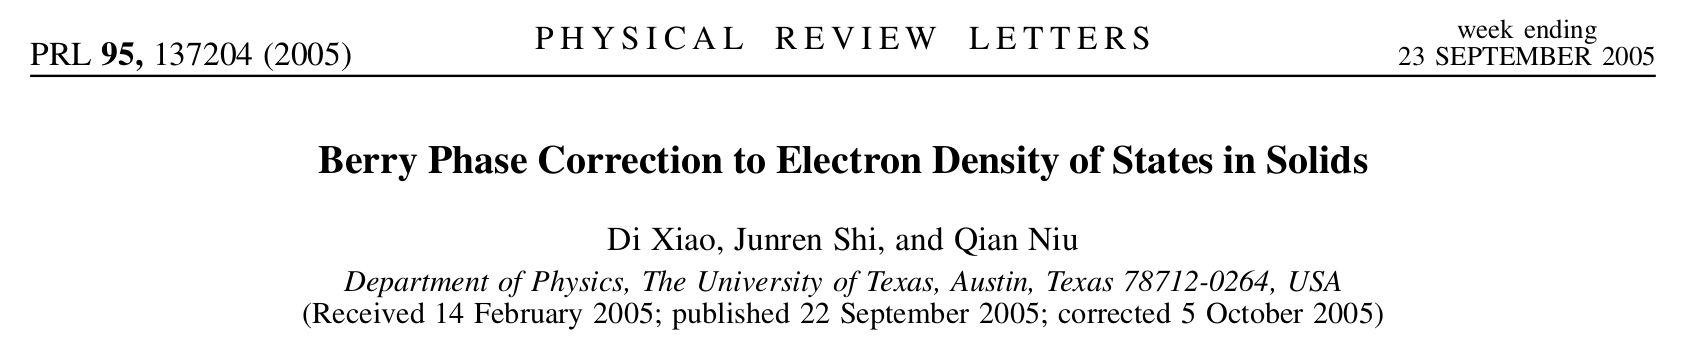
\includegraphics[width=\textwidth]{figure/classical-Morb.png}
      \end{tcolorbox}
      \ \\
      
      Combine the Eq. \eqref{eq::niuq} and Eq. \eqref{eq::xiaodi}, they find the total energy of the whole system can be written as, 
      \begin{equation}
        E_{\text{total}} = \sum_n\int^{\mu(\bm{B})}\frac{\mathrm{d}^3k}{(2\pi)^3}\; f_{n\bm{k}}\left(1 + \frac{e}{\hbar{}c}\bm{B}\cdot\bm{\Omega}_{n\bm{k}}\right)(E_{n\bm{k}}-\bm{m}_{n\bm{k}}\cdot\bm{B})
      \end{equation}
      
      Then the orbital magnetization can be directly calculated as, 
      \begin{subequations}
        \begin{align}
          \bm{M}_{\text{orb}} &= \nabla_{\bm{B}}E_{\text{total}} |_{\bm{B}=0} = \bm{M}_{\text{orb}}^{\text{MOM}} + \bm{M}_{\text{orb}}^{\text{DOS}}\\
          \bm{M}_{\text{orb}}^{\text{MOM}} &= \frac{e}{2\hbar{}c}\text{Im}\sum_n\int_{\text{BZ}}\frac{\mathrm{d}^3k}{(2\pi)^3}\; f_{n\bm{k}}\langle\nabla_{\bm{k}}u_{n\bm{k}}|\times(\widehat{H}_{\bm{k}}-E_{n\bm{k}})|\nabla_{\bm{k}}u_{n\bm{k}}\rangle\\
          \bm{M}_{\text{orb}}^{\text{DOS}} &= \frac{e}{2\hbar{}c}\text{Im}\sum_n\int_{\text{BZ}}\frac{\mathrm{d}^3k}{(2\pi)^3}\; f_{n\bm{k}}\langle\nabla_{\bm{k}}u_{n\bm{k}}|\times{}2(E_{n\bm{k}}-\mu_{0})|\nabla_{\bm{k}}u_{n\bm{k}}\rangle
        \end{align}
      \end{subequations}
    \end{frame}
    %-===================================================================-% 

    \section{Discussion}

    %+===================================================================+%
    \begin{frame}{Compare orbital magnetization \(\bm{M}_{\text{orb}}\) and polarization \(\bm{P}\)}\small
      \begin{block}{}
        Both of the \(\bm{M}_{\text{orb}}\) and \(\bm{P}\) comes from the ill-defined operator \(\widehat{\bm{r}}\), and because of which, have a close relation with the \purple{Berry connection}.
      \end{block}
      \begin{block}{}
        In the \(\bm{M}_{\text{orb}}\), we use \purple{\(\langle\psi_{\bm{k}}|\bm{r}\times\bm{v}|\psi_{\bm{k}}\rangle \to \langle\omega_{\bm{0}}|\bm{r}\times\bm{v}|\omega_{\bm{0}}\rangle\)} to sneak by the problem, while, in the \(\bm{P}\), \purple{\(\langle\psi_{\bm{k}}|\bm{r}|\psi_{\bm{k}}\rangle \to \langle\omega_{\bm{0}}|\bm{r}|\omega_{\bm{0}}\rangle\)} do the same.
      \end{block}
      \begin{block}{}
        Unlike \(\bm{P}\), which only involved the Bloch functions \(|u_{n\bm{k}}\rangle\), the \(\bm{M}_{\text{orb}}\) also \purple{need the Hamiltonlian}. \textcolor{gray}{E.g., if \(\widehat{H}\) is scaled by a multiplicative factor, \(\bm{M}_{\text{orb}}\) gets the same scaled, while \(\bm{P}\) remain invariant.}
      \end{block}
      \begin{columns}
        \begin{column}{0.68\textwidth}
          \begin{block}{}
            Unlike \(\bm{P}\), which is a ``valued lattice'', the \(\bm{M}_{\text{orb}}\) is \purple{single valued}. It can be understand from two perspectives,
            \begin{itemize}
              \item Solids allow the static charge on the surface, but do not allow surface charge accumulation.
              \item In nature, there are electric charges but no magnetic monopoles.
            \end{itemize}
          \end{block}
        \end{column}
        \begin{column}{0.3\textwidth}
          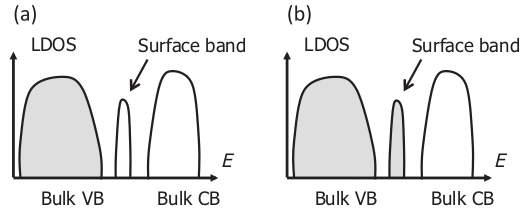
\includegraphics[width=\textwidth]{figure/P-surf.png}
        \end{column}
      \end{columns}
    \end{frame}
    %-===================================================================-% 

    %+===================================================================+%
    \begin{frame}{Theory beyond ``modern theory''}
      \begin{itemize}
        \item Finite-temperature system.\\
        \begin{tcolorbox}[beamer,width=0.6\textwidth,arc=0pt,boxsep=0.3pt,left=0pt,right=0pt,top=0pt,bottom=0pt]
          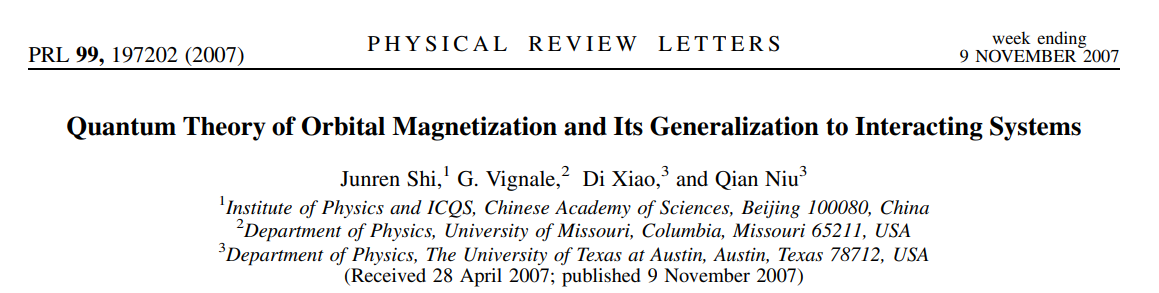
\includegraphics[width=\textwidth]{figure/Morb-temp.png}
        \end{tcolorbox}
        \item Calculate \(\bm{M}_{\text{orb}}\) in a pseudopotential context.\\
        \begin{tcolorbox}[beamer,width=0.6\textwidth,arc=0pt,boxsep=0.3pt,left=0pt,right=0pt,top=0pt,bottom=0pt]
          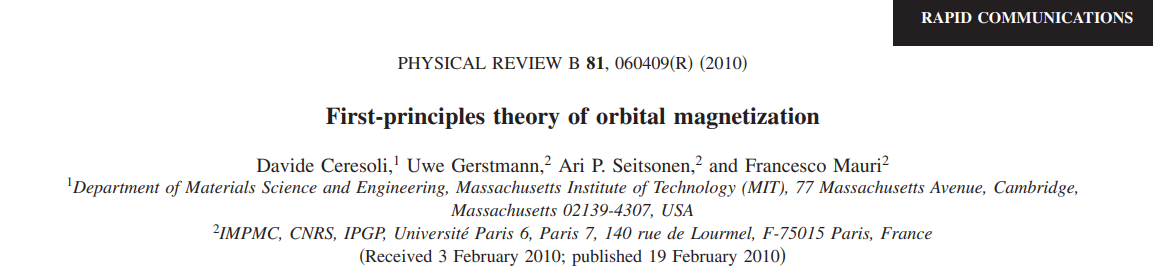
\includegraphics[width=\textwidth]{figure/Morb-DFT.png}
        \end{tcolorbox}
        \item Many-particle version \(\bm{M}_{\text{orb}}\).\\
        \begin{tcolorbox}[beamer,width=0.5\textwidth,arc=0pt,boxsep=0.3pt,left=0pt,right=0pt,top=0pt,bottom=0pt]
          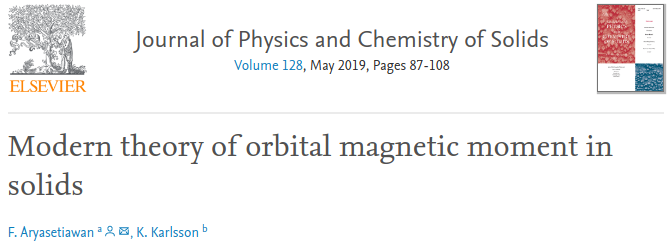
\includegraphics[width=\textwidth]{figure/Morb-mp.png}
        \end{tcolorbox}
      \end{itemize}
    \end{frame}
    %-===================================================================-% 

    %+===================================================================+%
    \begin{frame}{Total magnetization in solids}
      \begin{block}{Total magnetization in solids}
        The total magnetization of the system can be written as follow,
        \begin{subequations}\footnotesize
          \begin{align}
            \bm{M}_{\text{total}} &= \bm{M}_{\text{spin}} + \bm{M}_{\text{orb}}\\
            \bm{M}_{\text{spin}} &= \mu_{\text{B}}\frac{-g_s}{\hbar}\sum_n\int_{\text{BZ}}\frac{\mathrm{d}^3k}{(2\pi)^3}f_{n\bm{k}}\langle\psi_{n\bm{k}}|\widehat{\bm{S}}|\psi_{n\bm{k}}\rangle\\
            \bm{M}_{\text{orb}} &= \mu_{\text{B}}\frac{m_e}{\hbar^2}\sum_n\int_{\text{BZ}}\frac{\mathrm{d}^3k}{(2\pi)^3}f_{n\bm{k}}\text{Im}\langle\nabla_{\bm{k}}u_{n\bm{k}}|\times(\widehat{H}_{\bm{k}}+E_{n\bm{k}}-2\mu_{0})|\nabla_{\bm{k}}u_{n\bm{k}}\rangle
          \end{align}
        \end{subequations}
      \end{block}
      \begin{alertblock}{An interesting question}
        Why the \(\bm{M}_{\text{spin}}\) is often far large than (10 to 100 times) \(\bm{M}_{\text{orb}}\) in solids?
      \end{alertblock}
    \end{frame}
    %-===================================================================-%

    %+===================================================================+%
    \begin{frame}{Why \(\bm{M}_{\text{spin}}\) is often large than \(\bm{M}_{\text{orb}}\)?}\small
      The effective Hamiltonlian near the ground state:
      \begin{equation}
        \widehat{H}_{\text{eff}} = \begin{pmatrix}
          \widehat{H}_{\uparrow} & \widehat{W}_{\text{SOC}}\\
         \widehat{W}_{\text{SOC}} & \widehat{H}_{\downarrow}
         \end{pmatrix}, \;\;\; \widehat{W}_{\text{SOC}} \approx \lambda\widehat{\bm{L}}\cdot\widehat{\bm{S}}
      \end{equation}
      \begin{block}{Some personal arguments}
        \begin{itemize}
          \item In solid, the time-reversal symmetry (TRS) breaking in spin channels is common, for it is a requirement of fermions symmetry.
          \item The TRS breaking in orbital space is not as common as spin. Usually, orbits ``borrows'' the TRS breaking from spin space with the help of spin-orbit coupling (SOC).
          \item The orbital magnetization introduced via SOC may have the same magnitude order as SOC.
          \item There \textbf{are} ways to break the orbital TRS without SOC. In those cases, theoretically, the orbital magnetic moment can have a comparable value as spin's. \purple{(That is another long story...)}
        \end{itemize}
      \end{block}
    \end{frame}
    %-===================================================================-%

    \section{Summary}

    %+===================================================================+%
    \begin{frame}{Summary}
    \begin{block}{Summary}
      \begin{itemize}
        \item \(\bm{M}_{\text{total}} = \bm{M}_{\text{spin}} + \bm{M}_{\text{orb}}\). Often, the \(\bm{M}_{\text{spin}}\) accounts for a large proportion.
        \item The modern theory of oribtal magnetization gives,
        \begin{equation*}
          \bm{M}_{\text{orb}} = \frac{e}{2\hbar{}c}\text{Im}\sum_n\int_{\text{BZ}}\frac{\mathrm{d}^3k}{(2\pi)^3}f_{n\bm{k}}\langle\nabla_{\bm{k}}u_{n\bm{k}}|\times(\widehat{H}_{\bm{k}}+E_{n\bm{k}}-2\mu_{0})|\nabla_{\bm{k}}u_{n\bm{k}}\rangle
        \end{equation*}
        which is a single particle equation valid for both insulators and metals.
        \item Besides the trival edge state, the topological edge state also gives a term in the orbital magnetization.
        \item The same equation can also gain from the smei-classical theory. 
        \item The modern theory of orbital magnetization have a close relation with the modern theory of polarization.
      \end{itemize}
    \end{block}
    \end{frame}
    %-===================================================================-%
\end{document} 